\ifx\wholebook\relax \else
% ------------------------

\documentclass{article}
\usepackage[en]{../../../prelude}

\setcounter{page}{1}

\begin{document}

%--------------------------

% ================================================================
%                 COVER PAGE
% ================================================================

\title{Red-black tree, not so complex as it was thought}

\author{Larry~LIU~Xinyu
\thanks{{\bfseries Larry LIU Xinyu } \newline
  Email: liuxinyu95@gmail.com \newline}
  }

\maketitle
\fi

\markboth{Red black tree}{Elementary Algorithms}

\ifx\wholebook\relax
\chapter{Red-black tree, not so complex as it was thought}
\numberwithin{Exercise}{chapter}
\fi

% ================================================================
%                 Introduction
% ================================================================
\section{Introduction}
\label{introduction} \index{red-black tree}

\subsection{Exploit the binary search tree}
We showed the power of using binary search tree as a dictionary
to count the occurrence of every word in a book in previous chapter.

One may come to the idea to feed a yellow page book
\footnote{A telephone number contact list book} to a binary
search tree, and use it to look up the phone number for a contact.

By modifying a bit of the program for word occurrence counting
yields the following code.

\begin{lstlisting}
int main(int, char** ){
  ifstream f("yp.txt");
  map<string, string> dict;
  string name, phone;
  while(f>>name && f>>phone)
    dict[name]=phone;
  for(;;){
    cout<<"\nname: ";
    cin>>name;
    if(dict.find(name)==dict.end())
      cout<<"not found";
    else
      cout<<"phone: "<<dict[name];
  }
}
\end{lstlisting}

This program works well. However, if you replace the STL map
with the binary search tree introduced in previous chapter, the
performance will be bad, especially when you search some names such
as Zara, Zed, Zulu.

This is because the content of yellow page is typically listed
in lexicographic order. Which means the name list is in increase
order. If we try to insert a sequence of number 1, 2, 3, ..., $n$
to a binary search tree, we will get a tree like in Figure \ref{fig:unbalanced-tree}.

\begin{figure}[htbp]
       \centering
	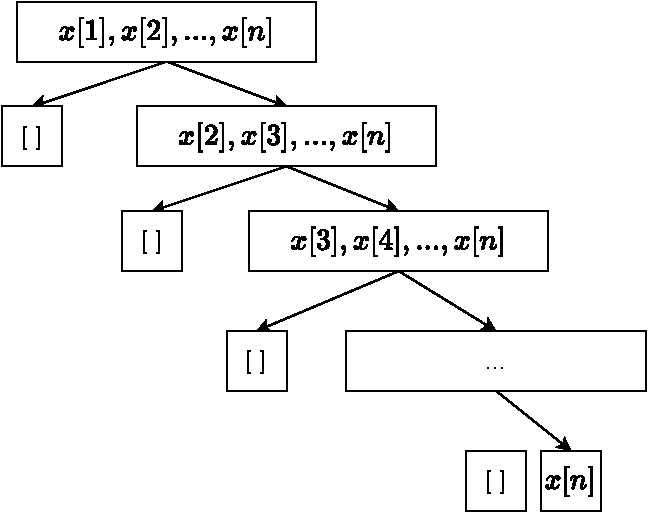
\includegraphics[scale=0.5]{img/unbalanced.ps}
        \caption{unbalanced tree} \label{fig:unbalanced-tree}
\end{figure}

This is extreme unbalanced binary search tree. The looking up performs
$O(h)$ for a tree with height $h$. In balanced case, we benefit from
binary search tree by $O(\lg n)$ search time. But in this extreme case,
the search time downgraded to $O(n)$. It's no better than a normal link-list.

\begin{Exercise}

\begin{itemize}
\item For a very big yellow page list, one may want to speed up the
dictionary building process by two concurrent tasks (threads or processes).
One task reads the name-phone pair from the head of the list, while the
other one reads from the tail. The building terminates when these
two tasks meet at the middle of the list. What will be the binary
search tree looks like after building? What if you split the
list more than two and use more tasks?

\item Can you find any more cases to exploit a binary search tree?
Please consider the unbalanced trees shown in figure
\ref{fig:unbalanced-trees}.
\end{itemize}

\end{Exercise}

\begin{figure}[htbp]
       \centering
       \subcaptionbox{}{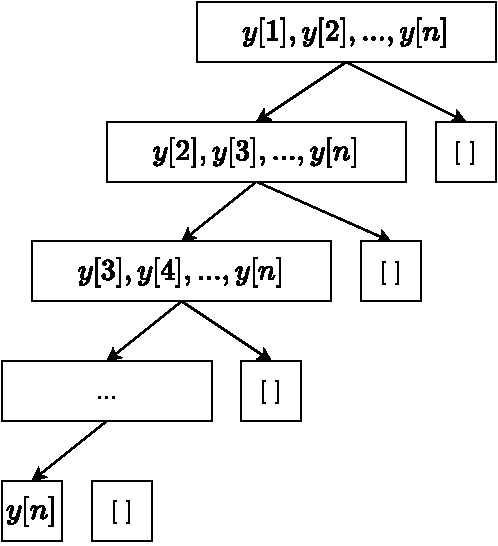
\includegraphics[scale=0.4]{img/unbalanced-2.ps}}
       \subcaptionbox{}{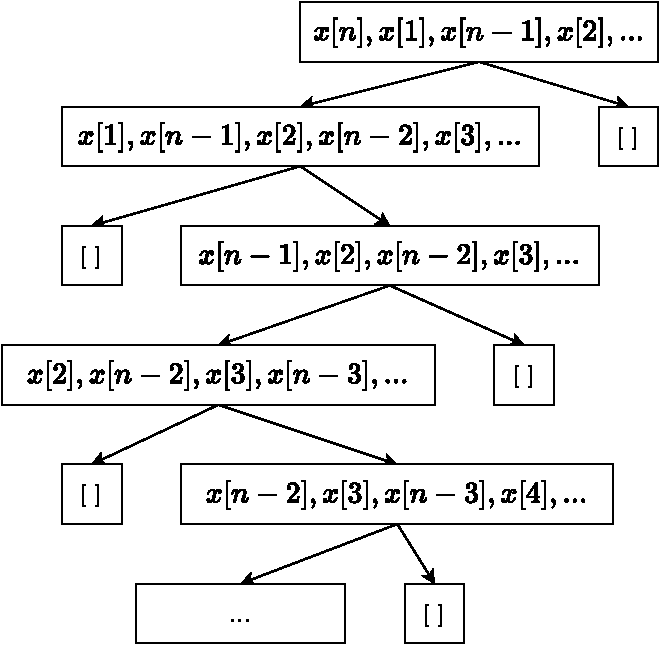
\includegraphics[scale=0.4]{img/unbalanced-zigzag.ps}} \\
       \subcaptionbox{}{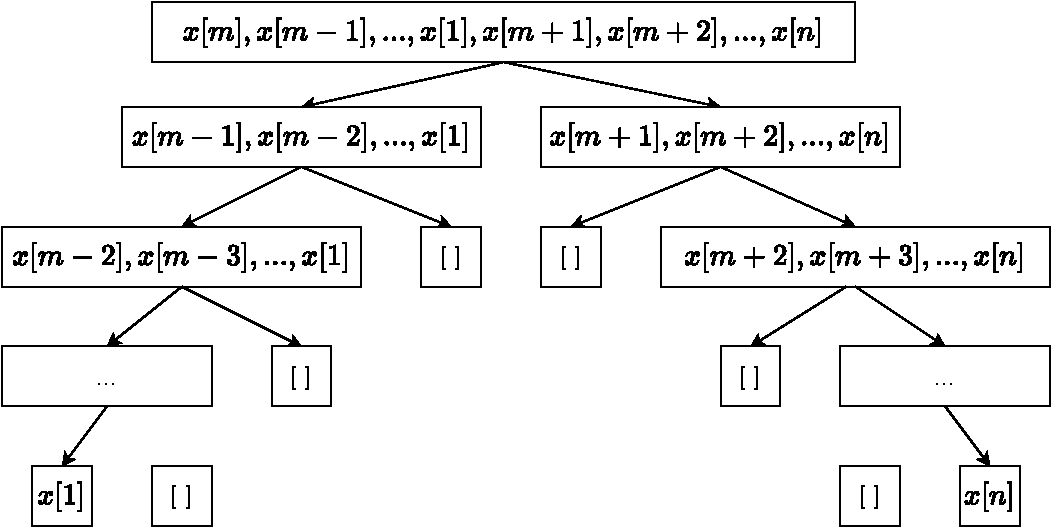
\includegraphics[scale=0.4]{img/unbalanced-3.ps}}
       \caption{Some unbalanced trees}
       \label{fig:unbalanced-trees}
\end{figure}

\subsection{How to ensure the balance of the tree}
In order to avoid such case, we can shuffle the input sequence by
randomized algorithm, such as described in Section 12.4 in \cite{CLRS}.
However, this method doesn't always work, for example the input is fed
from user interactively, and the tree need to be built and updated online.

There are many solutions people found to make binary search tree balanced.
Many of them rely on the rotation operations to the binary search tree.
Rotation operations change the tree structure while maintain the ordering
of the elements. Thus it can be used to improve the balance property of the binary
search tree.

In this chapter, we'll first introduce the red-black tree. It is one of the
most popular and widely used self-adjusting balanced
binary search tree. In next chapter, we'll introduce another intuitive solution, the AVL tree. In later chapter about binary heaps, we'll show another
interesting tree called splay tree, which can gradually adjust the the tree to make it
more and more balanced.

\subsection{Tree rotation}
\index{tree rotation}

\begin{figure}[htbp]
   \centering
   \setlength{\unitlength}{1cm}
   \begin{picture}(10, 4)
   \put(5, 2){$\Longleftrightarrow$}
   \subcaptionbox{}{\includegraphics[scale=0.4]{img/rotate-r.ps}}
   \subcaptionbox{}{\includegraphics[scale=0.4]{img/rotate-l.ps}}
   \end{picture}
   \\
   \begin{picture}(1, 0.5)\end{picture} %pad
   \caption{Tree rotation, `rotate-left' transforms the tree from left side to right side, and `rotate-right' does the inverse transformation.}
   \label{fig:tree-rotation}
\end{figure}

Tree rotation is a set of operations that can transform the tree structure
without changing the in-order traverse result. It based on the fact that
for a specified ordering, there are multiple binary search trees correspond to it.
Figure \ref{fig:tree-rotation} shows the tree rotation. For a binary search tree
on the left side, left rotate transforms it to the tree on the right, and right
rotate does the inverse transformation.

Although tree rotation can be realized in procedural way, there exists
simple functional definition by using pattern matching. Denote the non-empty tree as $T = (T_l, k, T_r)$, where $k$ is the key, and $T_l$, $T_r$ are left and right sub-trees.

\be
rotate_l(T) = \left \{
  \begin{array}
  {r@{\quad:\quad}l}
  ((a, X, b), Y, c) & T = (a, X, (b, Y, c)) \\
  T & otherwise
  \end{array}
\right .
\ee

\be
rotate_r(T) = \left \{
  \begin{array}
  {r@{\quad:\quad}l}
  (a, X, (b, Y, c)) & T = ((a, X, b), Y, c)) \\
  T & otherwise
  \end{array}
\right .
\ee

To perform tree rotation imperatively, we need set all fields of the node as the following.

\begin{algorithmic}[1]
\Function{Left-Rotate}{$T, x$}
  \State $p \gets$ \Call{Parent}{$x$}
  \State $y \gets$ \Call{Right}{$x$} \Comment{Assume $y \ne$ NIL}
  \State $a \gets$ \Call{Left}{$x$}
  \State $b \gets$ \Call{Left}{$y$}
  \State $c \gets$ \Call{Right}{$y$}
  \State \Call{Replace}{$x, y$}
  \State \Call{Set-Children}{$x, a, b$}
  \State \Call{Set-Children}{$y, x, c$}
  \If{$p = $ NIL}
    \State $T \gets y$
  \EndIf
  \State \Return $T$
\EndFunction

\Statex

\Function{Right-Rotate}{$T, y$}
  \State $p \gets$ \Call{Parent}{$y$}
  \State $x \gets$ \Call{Left}{$y$} \Comment{Assume $x \ne$ NIL}
  \State $a \gets$ \Call{Left}{$x$}
  \State $b \gets$ \Call{Right}{$x$}
  \State $c \gets$ \Call{Right}{$y$}
  \State \Call{Replace}{$y, x$}
  \State \Call{Set-Children}{$y, b, c$}
  \State \Call{Set-Children}{$x, a, y$}
  \If{$p = $ NIL}
    \State $T \gets x$
  \EndIf
  \State \Return $T$
\EndFunction
\end{algorithmic}

Where procedure \textproc{Replace}($x$, $y$), uses $y$ to replace $x$.

\begin{algorithmic}[1]
\Function{Replace}{$x, y$}
  \If{\Call{Parent}{$x$} = NIL}
    \If{$y \ne$ NIL}
      \Call{Parent}{$y$} $\gets$ NIL
    \EndIf
  \ElsIf{\textproc{Left}(\Call{Parent}{$x$}) $= x$}
    \State \textproc{Set-Left}(\Call{Parent}{$x$}, $y$)
  \Else
    \State \textproc{Set-Right}(\Call{Parent}{$x$}, $y$)
  \EndIf
  \State \Call{Parent}{$x$} $\gets$ NIL
\EndFunction
\end{algorithmic}

Procedure \textproc{Set-Children} assigns a pair of sub-trees
as the left and right children of a given node.

\begin{algorithmic}[1]
\Function{Set-Children}{$x, L, R$}
  \State \Call{Set-Left}{$x, L$}
  \State \Call{Set-Right}{$x, R$}
\EndFunction

\Statex

\Function{Set-Left}{$x, y$}
  \State \Call{Left}{$x$} $\gets y$
  \If{$y \ne$ NIL}
    \Call{Parent}{$y$} $\gets x$
  \EndIf
\EndFunction

\Statex

\Function{Set-Right}{$x, y$}
  \State \Call{Right}{$x$} $\gets y$
  \If{$y \ne$ NIL}
    \Call{Parent}{$y$} $\gets x$
  \EndIf
\EndFunction
\end{algorithmic}

Compare the imperative operations with the pattern matching functions,
we can found the latter focus on the structure change, while the
former focus on the rotation process. As the title of this
chapter indicated, red-black tree needn't be so complex as it
was thought. Many traditional algorithm text books use the
classic procedural treatment to the red-black tree. When insert or delete
keys, there are multiple cases with a series of node manipulation.
On the other hand, in functional settings, the algorithm turns to be intuitive and
simple, although there is some performance overhead.

Most of the content in this chapter is based on Chris Okasaki's
work in \cite{okasaki}.

% ================================================================
% Definition
% ================================================================
\section{Definition of red-black tree}
\index{red-black tree}

Red-black tree is a type of self-balancing binary search tree\cite{wiki}.
\footnote{Red-black tree is one of the equivalent form of 2-3-4 tree (see chapter
B-tree about 2-3-4 tree). That is to say, for any 2-3-4 tree, there is at least
one red-black tree has the same data order.} By using color changing and rotation,
red-black tree provides a very simple and straightforward way to keep
the tree balanced.

For a binary search tree, we can augment the nodes with a color field, a node
can be colored either red or black. We call a binary search tree red-black tree
if it satisfies the following 5 properties(\cite{CLRS} pp273).
\index{red-black tree!red-black properties}

\begin{enumerate}
\item Every node is either red or black.
\item The root is black.
\item Every leaf (NIL) is black.
\item If a node is red, then both its children are black.
\item For each node, all paths from the node to descendant leaves contain the same number of black nodes.
\end{enumerate}

Why this 5 properties can ensure the red-black tree is well balanced?
Because they have a key characteristic, the longest path from root to
a leaf can't be as 2 times longer than the shortest path.

Consider the 4-th property. It means there can't be two adjacent
red nodes. so the shortest path only contains black nodes, any path
that is longer than the shortest one has interval red nodes. According to
property 5, all paths have the same number of black nodes,
it finally ensures there can't be any path that is 2 times longer than
others\cite{wiki}. Figure \ref{fig:rbt-example-with-nil} shows a red-black tree example.

\begin{figure}[htbp]
       \begin{center}
	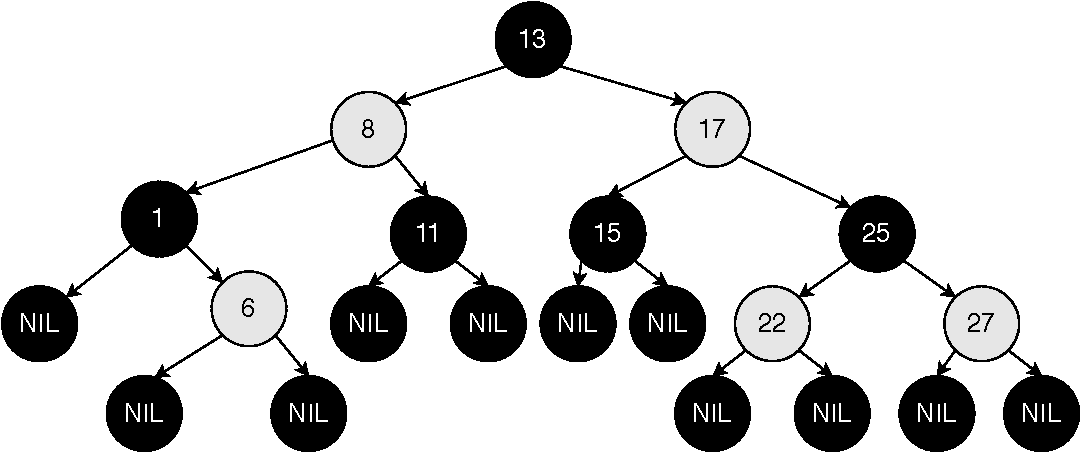
\includegraphics[scale=0.6]{img/rbt-example-with-nil.ps}
        \caption{A red-black tree} \label{fig:rbt-example-with-nil}
       \end{center}
\end{figure}

As all NIL nodes are black, people often omit them when draw red-black tree. Figure \ref{fig:rbt-example} gives the corresponding tree that hides all the NIL nodes.

\begin{figure}[htbp]
       \begin{center}
	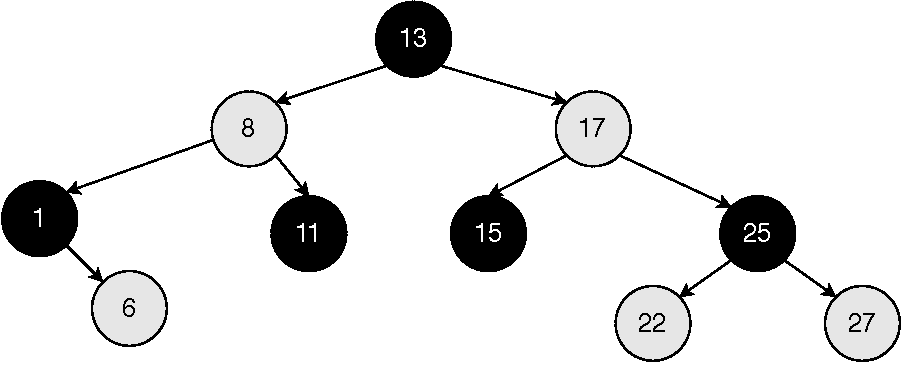
\includegraphics[scale=0.6]{img/rbt-example.ps}
        \caption{The red-black tree with all NIL nodes hidden.} \label{fig:rbt-example}
       \end{center}
\end{figure}

All read operations such as search, find the min/max, are same as the
binary search tree. The insertion and deletion are special for the red-black tree.

Many implementation of set or map container are based on red-black tree.
One example is the C++ Standard library (STL)\cite{sgi-stl}.

For the data layout, the only change is the color
color information need be augmented to binary search tree.
This can be represented as a data field. Like the below C++ example.

\lstset{language=C++}
\begin{lstlisting}
enum Color {Red, Black};

template <class T>
struct node{
  Color color;
  T key;
  node* left;
  node* right;
  node* parent;
};
\end{lstlisting}

In functional settings, we can add the color information
in constructors, below is the Haskell example of red-black tree
definition.

\lstset{language=Haskell}
\begin{lstlisting}
data Color = R | B
data RBTree a = Empty
              | Node Color (RBTree a) a (RBTree a)
\end{lstlisting}

\begin{Exercise}

\begin{itemize}
\item Can you prove that a red-black tree with $n$ nodes has
height at most $2 \lg (n+1)$?
\end{itemize}

\end{Exercise}

% ================================================================
%                 Insertion
% ================================================================
\section{Insertion}
\index{red-black tree!insertion}

The tree may be unblanced if a new node is inserted with the method we
used for the binary search tree. In order to maintain the red-black properties,
we need do some fixing after insertion.

When insert a new key, we can always insert it as a
red node. As far as the new inserted node isn't the root of the tree,
we can keep all properties except the 4-th one as it may bring two
adjacent red nodes.

There are both functional and procedural fixing methods.
One is intuitive but has some overhead, the other is a bit complex but has
higher performance. In this chapter, we focus on the functional approach
to show how easy a red-black tree insertion algorithm can be realized.
The traditional procedural method will be given for comparison purpose.

As described by Chris Okasaki, there are total 4 cases which violate property 4.
All of them has 2 adjacent red nodes. However, they have a uniformed structure
after fixing\cite{okasaki} as shown in figure \ref{fig:insert-fix}.

\begin{figure}[htbp]
   \begin{center}
     \setlength{\unitlength}{1cm}
     \begin{picture}(15, 15)
        % arrows
        \put(4.5, 9.5){\vector(1, -1){1}}
        \put(4.5, 5){\vector(1, 1){1}}
        \put(10, 9.5){\vector(-1, -1){1}}
        \put(10, 5){\vector(-1, 1){1}}
        % graphics
	\put(0, 7){\includegraphics[scale=0.5]{img/insert-ll.ps}}
        \put(0, 0){\includegraphics[scale=0.5]{img/insert-lr.ps}}
        \put(7, 7){\includegraphics[scale=0.5]{img/insert-rr.ps}}
        \put(8.5, 0){\includegraphics[scale=0.5]{img/insert-rl.ps}}
        \put(2, 5){\includegraphics[scale=0.5]{img/insert-fixed.ps}}
      \end{picture}
     \caption{4 cases for balancing a red-black tree after insertion} \label{fig:insert-fix}
  \end{center}
\end{figure}

Note that this transformation will move the redness one level up.
During the bottom-up recursive fixing, the last step will make
the root node red. According to property 2, root is always black,
thus we need finally fix to revert the root color to black.

Observing that the 4 cases and the fixed result have strong patterns,
the fixing function can be defined by using the similar
method we mentioned in tree rotation. Denote the color of a node as
$\mathcal{C}$, it has two values: black $\mathcal{B}$, and red$\mathcal{R}$.
A none empty tree can be represented as $T = (\mathcal{C}, T_l, k, T_r)$.

\be
balance(T) = \left \{
  \begin{array}
  {r@{\quad:\quad}l}
  (\mathcal{R}, (\mathcal{B}, A, x, B), y, (\mathcal{B}, C, z, D)) & match(T) \\
  T & otherwise
  \end{array}
\right .
\ee

where function $match()$ tests if a tree mathes one of the 4 possible patterns as the following.

\[
match(T) = \left \{ T = \begin{array}{l}
         (\mathcal{B}, (\mathcal{R}, (\mathcal{R}, A, x, B), y, C), z, D) \lor \\
         (\mathcal{B}, (\mathcal{R}, A, x, (\mathcal{R}, B, y, C), z, D)) \lor \\
         (\mathcal{B}, A, x, (\mathcal{R}, B, y, (\mathcal{R}, C, z, D))) \lor \\
         (\mathcal{B}, A, x, (\mathcal{R}, (\mathcal{R}, B, y, C), z, D)) \\
         \end{array} \right \}
\]

With function $balance(T)$ defined, we can modify the binary search tree
insertion functions to make it work for red-black tree.

\be
insert(T, k) = makeBlack(ins(T, k))
\ee

where

\be
ins(T, k) = \left \{
  \begin{array}
  {r@{\quad:\quad}l}
  (\mathcal{R}, \phi, k, \phi) & T = \phi \\
  balance((ins(T_l, k), k', T_r)) & k < k' \\
  balance((T_l, k', ins(T_r, k))) & otherwise
  \end{array}
\right.
\ee

If the tree is empty, then a new red node with $k$ as the key is created; otherwise, denote the children and the key as $T_l$, $T_r$, and $k'$, we compare $k$ and $k'$ and recursively insert $k$ to a child. Function $balance$ is called after that, and the root is re-colored black finally.

\be
makeBlack(T) = (\mathcal{B}, T_l, k, T_r)
\ee

Summarize the above functions and use language supported pattern matching
features, we can come to the following Haskell program.

\lstset{language=Haskell}
\begin{lstlisting}
insert t x = makeBlack $ ins t where
    ins Empty = Node R Empty x Empty
    ins (Node color l k r)
        | x < k     = balance color (ins l) k r
        | otherwise = balance color l k (ins r) --[3]
    makeBlack(Node _ l k r) = Node B l k r

balance B (Node R (Node R a x b) y c) z d =
                Node R (Node B a x b) y (Node B c z d)
balance B (Node R a x (Node R b y c)) z d =
                Node R (Node B a x b) y (Node B c z d)
balance B a x (Node R b y (Node R c z d)) =
                Node R (Node B a x b) y (Node B c z d)
balance B a x (Node R (Node R b y c) z d) =
                Node R (Node B a x b) y (Node B c z d)
balance color l k r = Node color l k r
\end{lstlisting} %$

Note that the 'balance' function is changed a bit from the original
definition. Instead of passing the tree, we pass
the color, the left child, the key and the right child to it.
This can save a pair of `boxing' and 'un-boxing' operations.

This program doesn't handle the case of duplicated keys. we can
either overwrite the key or drop the duplicated one.
Another option is to augment the data with a linked list(\cite{CLRS}, pp269).

Figure \ref{fig:insert-example} shows two red-black trees
built from feeding list 11, 2, 14, 1, 7, 15, 5, 8, 4 and 1, 2, ..., 8. The tree is well balanced even if we input an ordered list.

\begin{figure}[htbp]
  \centering
  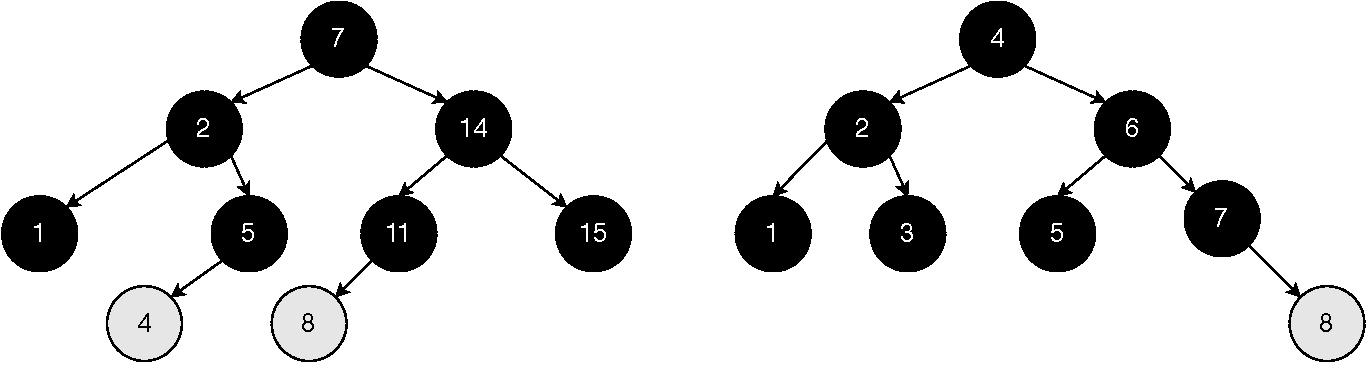
\includegraphics[scale=0.5]{img/insert-haskell.ps}
  \caption{insert results generated from two sequences of keys.} \label{fig:insert-example}
\end{figure}

This algorithm shows great simplicity by summarizing the uniform pattern
from the four different unbalanced cases. It is expressive over
the traditional tree rotation approach, that even in programming languages
which don't support pattern matching, the algorithm can still be
implemented by manually check the pattern. A Scheme/Lisp program
is available along with this book can be referenced as an example.

The insertion algorithm takes $O(\lg n)$ time to insert a key to
a red-black tree which has $n$ nodes.

\begin{Exercise}

\begin{itemize}
\item Write a program in an imperative language, such as
C, C++ or python to realize the same algorithm in this
section. Note that, because there is no language supported
pattern matching, you need to test the 4 different cases
manually.
\end{itemize}

\end{Exercise}

% ================================================================
%                 Deletion
% ================================================================

\section{Deletion}
\index{red-black tree!deletion}

Remind the deletion section in binary search tree. Deletion is
`imperative only' for red-black tree as well. In many cases,
the tree is often built just one time, and then
performs looking up frequently\cite{okasaki-blog}.

The purpose of this section is to show that red-black
tree deletion is possible in purely functional settings,
although it actually rebuilds the tree because trees are
read only in terms of purely functional data structure\footnote{Actually, the common part of the tree is reused. Most functional programming environments support this persistent feature.}.
In real world, it's up to the user (i.e. the
programmer) to adopt the proper solution. One option is to mark
the node be deleted with a flag, and later rebuild the tree
when the number of deleted nodes exceeds 50\%.

Deletion is more complex than insertion in both functional and
imperative settings, as there are more cases to fix.
Deletion may also violate the red black tree properties,
so we need fix it after the normal deletion as described
in binary search tree.

The problem only happens if you try to
delete a black node, because it will violate the last property
of red-black tree. The number of black
node in the path decreases so not all the paths contain the
same number of black node.

When delete a black node, we can resume the last red-black property
by introducing a 'doubly-black' concept(\cite{CLRS}, pp290). It means
that the although the node is deleted, the blackness is kept
by storing it in the parent node. If the parent node is red,
it turns to black, However, if it's already black, it
turns to `doubly-black'.

In order to express the 'doubly-black node', The definition
need some modification accordingly.

\lstset{language=Haskell}
\begin{lstlisting}
data Color = R | B | BB -- BB: doubly black for deletion
data RBTree a = Empty | BBEmpty -- doubly black empty
              | Node Color (RBTree a) a (RBTree a)
\end{lstlisting}

When deleting a node, we first perform the same binary search tree deleting
algorithm. After that, if the node to be sliced out is black, we
need fix the tree to keep the red-black properties. The
delete function is defined as the following.

\be
delete(T, k) = blackenRoot(del(T, k))
\ee

where

\be
del(T, k) = \left \{
  \begin{array}
  {r@{\quad:\quad}l}
  \phi & T = \phi \\
  fixBlack^2((\mathcal{C}, del(T_l, k), k', T_r)) & k < k' \\
  fixBlack^2((\mathcal{C}, T_l, k', del(T_r, k))) & k > k' \\
  \left \{
    \begin{array}{r@{\quad:\quad}l}
    mkBlk(T_r) & \mathcal{C} = \mathcal{B} \\
    T_r & otherwise
    \end{array}
  \right. & T_l = \phi \\
  \left \{
    \begin{array}{r@{\quad:\quad}l}
    mkBlk(T_l) & \mathcal{C} = \mathcal{B} \\
    T_l & otherwise
    \end{array}
  \right.  & T_r = \phi \\
  fixBlack^2((\mathcal{C}, T_l, k'', del(T_r, k''))) & otherwise
  \end{array}
\right.
\ee

The real deleting happens inside function $del$.
For the trivial case, that the tree is empty, the deletion
result is $\phi$; If the key to be deleted is less
than the key of the current node, we recursively
perform deletion on its left sub-tree; if it is bigger
than the key of the current node, then we recursively
delete the key from the right sub-tree; Because it
may bring doubly-blackness, so we need fix it.

If the key to be deleted is equal to the key of the
current node, we need splice it out. If one of its
children is empty, we just replace the node by
the other one and reserve the blackness of this
node. otherwise we cut and past the minimum
element $k''=min(T_r)$ from the right sub-tree.

Function $delete$ just forces the result tree of $del$
to have a black root. This is realized by function
$blackenRoot$.

\be
blackenRoot(T) = \left \{
  \begin{array}
  {r@{\quad:\quad}l}
  \phi & T = \phi \\
  (\mathcal{B}, T_l, k, T_r) & otherwise \\
  \end{array}
\right .
\ee

The $blackenRoot(T)$ function is almost same as the $makeBlack(T)$ function defined for insertion
except for the case of empty tree. This is only valid in
deletion, because insertion can't result an empty tree,
while deletion may.

Function $mkBlk$ is defined to reserved the blackness
of a node. If the node to be sliced isn't black, this function
won't be applied, otherwise, it turns a red node to black
and turns a black node to doubly-black. This function
also marks an empty tree $\phi$ to doubly-black empty $\Phi$.

\be
mkBlk(T) = \left \{
  \begin{array}
  {r@{\quad:\quad}l}
  \Phi & T = \phi \\
  (\mathcal{B}, T_l, k, T_r) & \mathcal{C} = \mathcal{R} \\
  (\mathcal{B}^2, T_l, k, T_r) & \mathcal{C} = \mathcal{B} \\
  T & otherwise
  \end{array}
\right .
\ee

where $\mathcal{B}^2$ denotes the doubly-black color.

Summarizing the above functions yields the following Haskell
program.

\begin{lstlisting}
delete t x = blackenRoot(del t x) where
    del Empty _ = Empty
    del (Node color l k r) x
        | x < k = fixDB color (del l x) k r
        | x > k = fixDB color l k (del r x)
        -- x == k, delete this node
        | isEmpty l = if color==B then makeBlack r else r
        | isEmpty r = if color==B then makeBlack l else l
        | otherwise = fixDB color l k' (del r k') where k'= min r
    blackenRoot (Node _ l k r) = Node B l k r
    blackenRoot _ = Empty

makeBlack (Node B l k r) = Node BB l k r -- doubly black
makeBlack (Node _ l k r) = Node B l k r
makeBlack Empty = BBEmpty
makeBlack t = t
\end{lstlisting}

The final attack to the red-black tree deletion algorithm is to
realize the $fixBlack^2$ function. The purpose of this function
is to eliminate the `doubly-black' colored node by rotation and
color changing. There are three cases. In every case, the doubly black
node can either be normal node, or doubly black empty node $\Phi$.
Let's examine these three cases one by one.

\subsection{The sibling of the doubly black node is black, and it has one red child}

In this situation, we can fix the doubly-blackness with one rotation.
Actually there are 4 different sub-cases, all of them can be transformed
to one uniformed pattern. They are shown in the figure \ref{fig:del-case1}.

\begin{figure}[htbp]
   \centering
   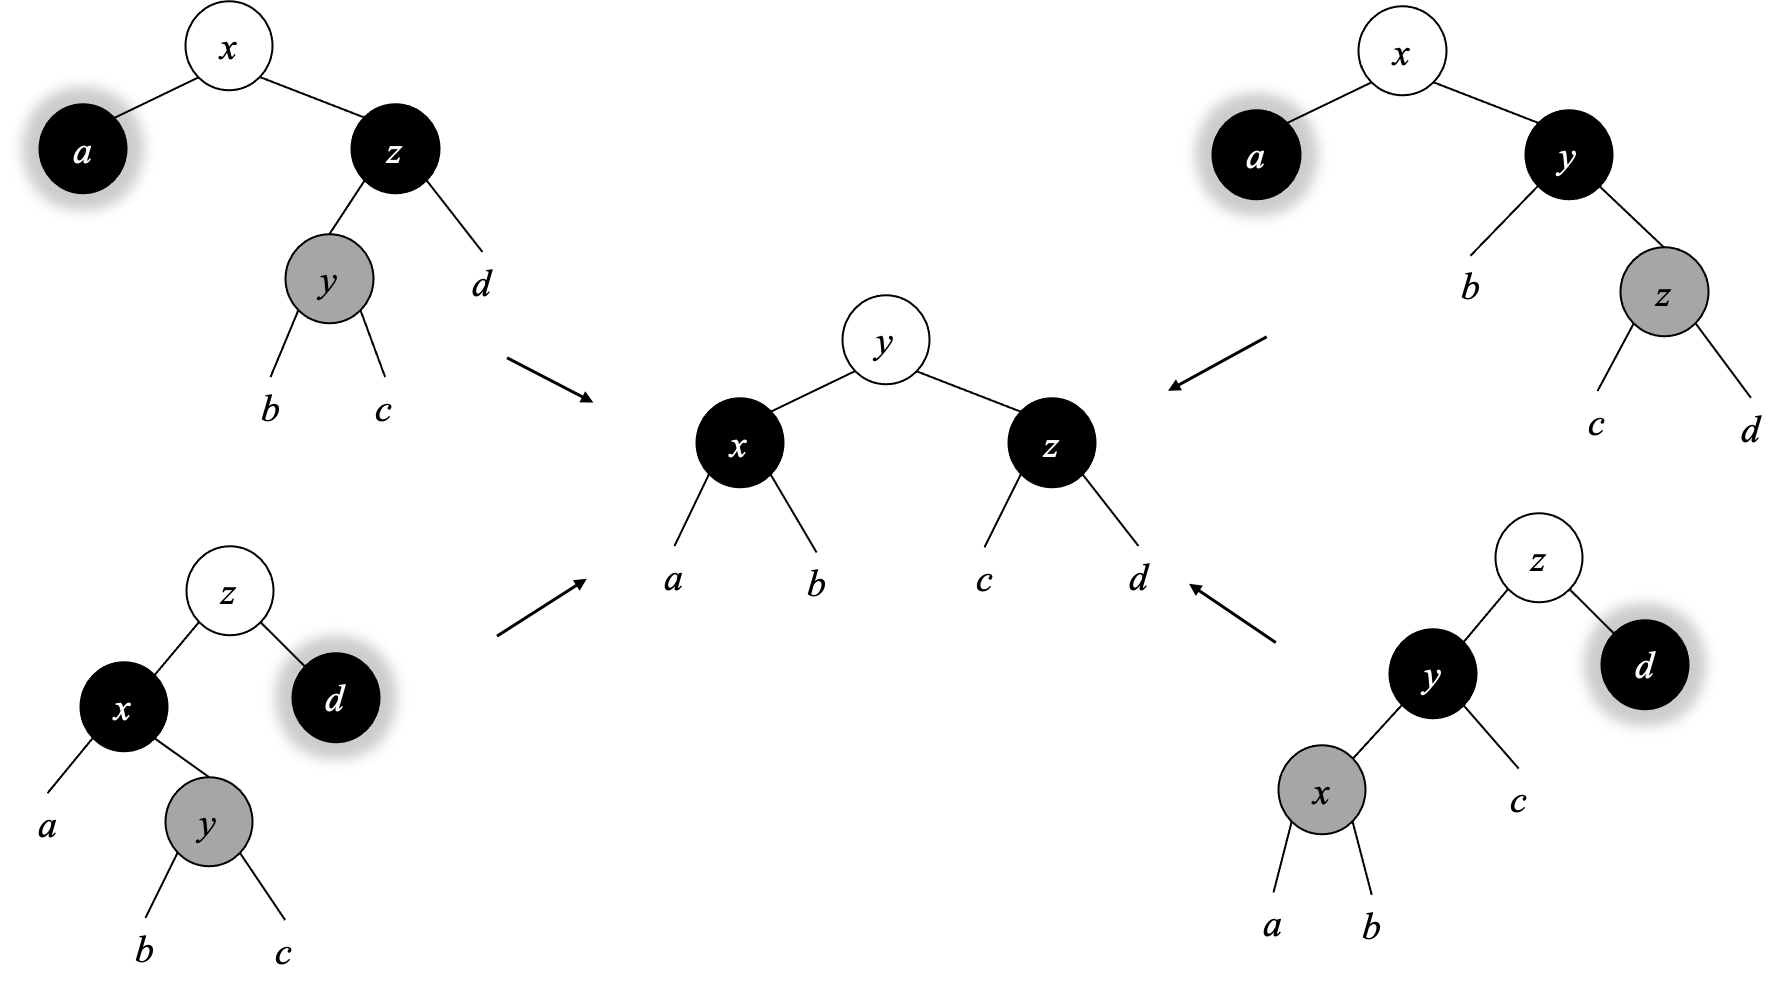
\includegraphics[scale=0.4]{img/del-case1.eps}
   \caption{Fix the doubly black by rotation, the sibling of the doubly-black node is black, and it has one red child.} \label{fig:del-case1}
\end{figure}

The handling of these 4 sub-cases can be realized with pattern matching.

\be
fixBlack^2(T) = \left \{
  \begin{array}
  {r@{\quad:\quad}l}
  (\mathcal{C}, (\mathcal{B}, mkBlk(A), x, B), y, (\mathcal{B}, C, z, D)) & p 1.1 \\
  (\mathcal{C}, (\mathcal{B}, A, x, B), y, (\mathcal{B}, C, z, mkBlk(D))) & p 1.2 \\
  \end{array}
\right .
\label{eq:db-case-1}
\ee

where $p 1.1$ and $p 1.2$ each represent 2 patterns as the following.

\[
p 1.1 : \left \{ \begin{array}{l}
  T = (\mathcal{C}, A, x, (\mathcal{B}, (\mathcal{R}, B, y, C), z, D)) \land color(A) = \mathcal{B}^2 \\
  \lor \\
  T = (\mathcal{C}, A, x, (\mathcal{B}, B, y, (\mathcal{R}, C, z, D))) \land color(A) = \mathcal{B}^2
  \end{array} \right \}
\]

\[
p 1.2 : \left \{ \begin{array}{l}
  T = (\mathcal{C}, (\mathcal{B}, A, x, (\mathcal{R}, B, y, C)), z, D) \land color(D) = \mathcal{B}^2 \\
  \lor \\
  T = (\mathcal{C}, (\mathcal{B}, (\mathcal{R}, A, x, B), y, C), z, D) \land color(D) = \mathcal{B}^2
  \end{array} \right \}
\]

If the doubly black node is a doubly black empty node $\Phi$, it can be changed back to normal empty node after the above operation. We can add the doubly black empty node handling on top of the (\ref{eq:db-case-1}).

\be
fixBlack^2(T) = \left \{
  \begin{array}
  {r@{\quad:\quad}l}
  (\mathcal{C}, (\mathcal{B}, mkBlk(A), x, B), y, (\mathcal{B}, C, z, D)) & p 1.1 \\
  (\mathcal{C}, (\mathcal{B}, \phi, x, B), y, (\mathcal{B}, C, z, D)) & p 1.1' \\
  (\mathcal{C}, (\mathcal{B}, A, x, B), y, (\mathcal{B}, C, z, mkBlk(D))) & p 1.2 \\
  (\mathcal{C}, (\mathcal{B}, A, x, B), y, (\mathcal{B}, C, z, \phi)) & p 1.2' \\
  \end{array}
\right .
\label{eq:db-case-1a}
\ee

Where patter $p 1.1'$ and $p 1.2'$ are defined as below:

\[
p 1.1' : \left \{ \begin{array}{l}
  T = (\mathcal{C}, \Phi, x, (\mathcal{B}, (\mathcal{R}, B, y, C), z, D)) \\
  \lor \\
  T = (\mathcal{C}, \Phi, x, (\mathcal{B}, B, y, (\mathcal{R}, C, z, D)))
  \end{array} \right \}
\]

\[
p 1.2' : \left \{ \begin{array}{l}
  T = (\mathcal{C}, (\mathcal{B}, A, x, (\mathcal{R}, B, y, C)), z, \Phi) \\
  \lor \\
  T = (\mathcal{C}, (\mathcal{B}, (\mathcal{R}, A, x, B), y, C), z, \Phi)
  \end{array} \right \}
\]

\subsection{The sibling of the doubly-black node is red}
In this case, we can rotate the tree to it to pattern $p 1.1$ or $p 1.2$.
Figure \ref{fig:del-case2} shows about it.

\begin{figure}[htbp]
  \centering
  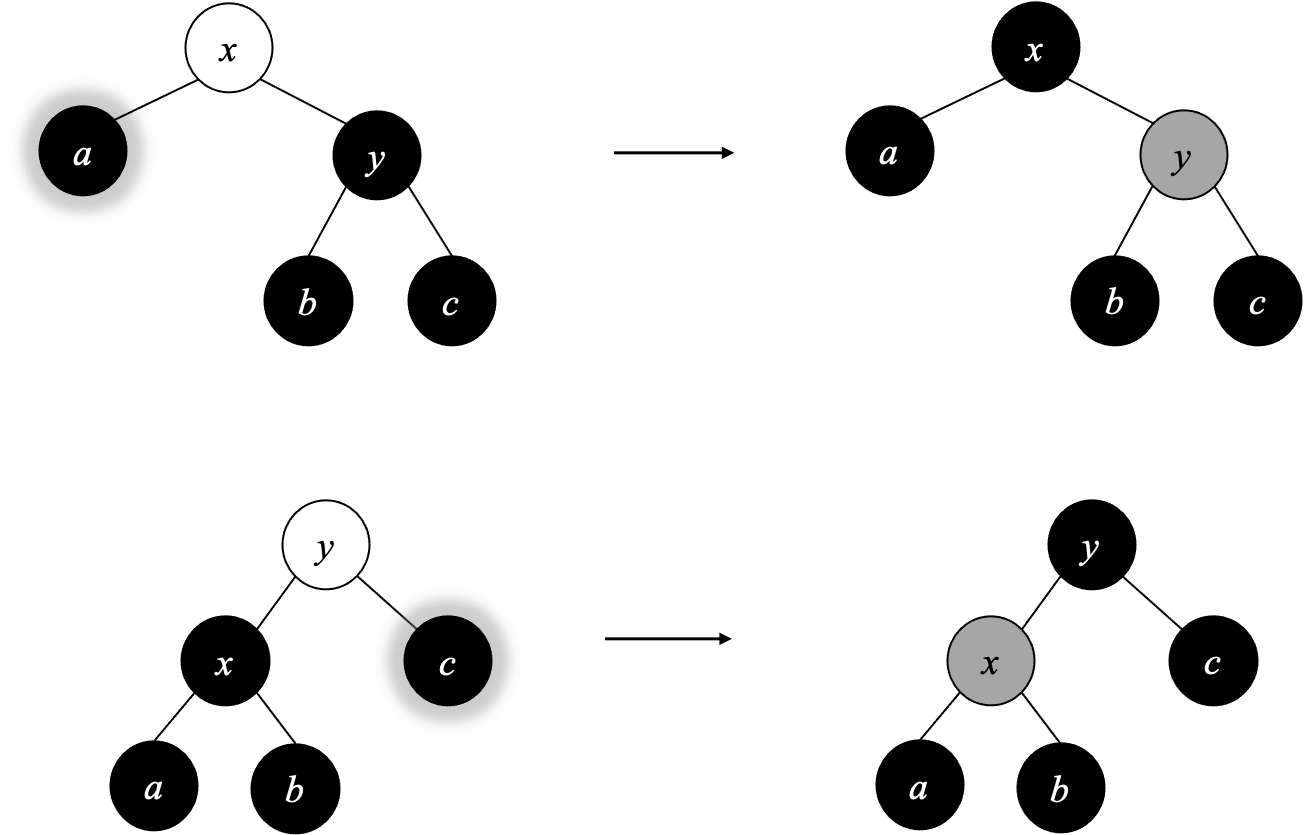
\includegraphics[scale=0.4]{img/del-case3.eps}
  \caption{The sibling of the doubly-black node is red.} \label{fig:del-case2}
\end{figure}

We can add this case on top of (\ref{eq:db-case-1a}) to gain (\ref{eq:db-case-2}).

\be
fixBlack^2(T) = \left \{
  \begin{array}
  {r@{\quad:\quad}l}
  ... & ... \\
  fixBlack^2(\mathcal{B}, fixBlack^2((\mathcal{R}, A, x, B), y, C) & p 2.1 \\
  fixBlack^2(\mathcal{B}, A, x, fixBlack^2((\mathcal{R}, B, y, C)) & p 2.2 \\
  T & otherwise
  \end{array}
\right .
\label{eq:db-case-2}
\ee

where $p 2.1$ and $p 2.2$ are two patterns as the following.

\[
p 2.1 : \{ color(T) = \mathcal{B} \land color(T_l) = \mathcal{B}^2 \land color(T_r) = \mathcal{R} \}
\]

\[
p 2.2 : \{ color(T) = \mathcal{B} \land color(T_l) = \mathcal{R} \land color(T_r) = \mathcal{B}^2 \}
\]

\subsection{The sibling of the doubly-black node, and its two children are all black}
In this case, we can change the color of the sibling node to red; turn the
doubly-black node to black and propagate the doubly-blackness one level
up to the parent node as shown in figure \ref{fig:del-case3}. There are two
symmetric sub-cases.

\begin{figure}[htbp]
  \centering
  \setlength{\unitlength}{1cm}
  \begin{picture}(10, 4)
  \put(5, 2){$\Longrightarrow$}
  \subcaptionbox{Color of $x$ can be either black or red.}{\includegraphics[scale=0.4]{img/case2-a.ps}}
  \subcaptionbox{If $x$ was red, then it becomes black, otherwise, it becomes doubly-black.}{\includegraphics[scale=0.4]{img/case2-a1.ps}}
  \end{picture}
  \\
  \begin{picture}(10, 5)
  \put(5, 2){$\Longrightarrow$}
  \subcaptionbox{Color of $y$ can be either black or red.}{\includegraphics[scale=0.4]{img/case2-b.ps}}
  \subcaptionbox{If $y$ was red, then it becomes black, otherwise, it becomes doubly-black.}{\includegraphics[scale=0.4]{img/case2-b1.ps}}
  \end{picture}
  \\
  \begin{picture}(1, 0.5)\end{picture} %pad
  \caption{propagate the blackness up.} \label{fig:del-case3}
\end{figure}

We go on adding this fixing after formula (\ref{eq:db-case-2}).

\be
fixBlack^2(T) = \left \{
  \begin{array}
  {r@{\quad:\quad}l}
  ... & ... \\
  mkBlk((\mathcal{C}, mkBlk(A), x, (\mathcal{R}, B, y, C))) & p 3.1 \\
  mkBlk((\mathcal{C}, (\mathcal{R}, A, x, B), y, mkBlk(C))) & p 3.2 \\
  ... & ...
  \end{array}
\right .
\label{eq:db-case-3}
\ee

where $p 3.1$ and $p 3.2$ are two patterns as below.

\[
p 3.1 : \left \{ \begin{array}{l}
  T = (\mathcal{C}, A, x, (\mathcal{B}, B, y, C)) \land \\
  color(A) = \mathcal{B}^2 \land color(B) = color(C) = \mathcal{B}
  \end{array} \right \}
\]

\[
p 3.2 : \left \{ \begin{array}{l}
  T = (\mathcal{C}, (\mathcal{B}, A, x, B), y, C) \land \\
  color(C) = \mathcal{B}^2 \land color(A) = color(B) = \mathcal{B}
  \end{array} \right \}
\]

If the doubly black node is doubly black empty node $\Phi$, it can be changed
back to normal empty node after re-coloring. We add the doubly black empty node
handling to (\ref{eq:db-case-3}) as below.

\be
fixBlack^2(T) = \left \{
  \begin{array}
  {r@{\quad:\quad}l}
  ... & ... \\
  mkBlk((\mathcal{C}, mkBlk(A), x, (\mathcal{R}, B, y, C))) & p 2.1 \\
  mkBlk((\mathcal{C}, \phi, x, (\mathcal{R}, B, y, C))) & p 2.1' \\
  mkBlk((\mathcal{C}, (\mathcal{R}, A, x, B), y, mkBlk(C))) & p 2.2 \\
  mkBlk((\mathcal{C}, (\mathcal{R}, A, x, B), y, \phi)) & p 2.2' \\
  ... & ...
  \end{array}
\right .
\label{eq:db-case-3a}
\ee

Where pattern $p 3.1'$ and $p 3.2'$ are defined as the following.

\[
p 3.1' : \left \{ \begin{array}{l}
  T = (\mathcal{C}, \Phi, x, (\mathcal{B}, B, y, C)) \land \\
  color(B) = color(C) = \mathcal{B}
  \end{array} \right \}
\]

\[
p 3.2' : \left \{ \begin{array}{l}
  T = (\mathcal{C}, (\mathcal{B}, A, x, B), y, \Phi) \land \\
  color(A) = color(B) = \mathcal{B}
  \end{array} \right \}
\]

Fixing the doubly-black node with all above different cases is a recursive function.
There are two termination conditions. One contains pattern $p 1.1$ and $p 1.2$,
The doubly-black node was eliminated. The other cases may continuously propagate the
doubly-blackness from bottom to top till the root.
Finally the algorithm marks the root node as black anyway. The doubly-blackness will be
removed.

Put formula (\ref{eq:db-case-1a}), (\ref{eq:db-case-2}), and (\ref{eq:db-case-3a})
together, we can write the final Haskell program.

\begin{lstlisting}
-- the sibling is black, and it has one red child
fixDB color a@(Node BB _ _ _) x (Node B (Node R b y c) z d)
      = Node color (Node B (makeBlack a) x b) y (Node B c z d)
fixDB color BBEmpty x (Node B (Node R b y c) z d)
      = Node color (Node B Empty x b) y (Node B c z d)
fixDB color a@(Node BB _ _ _) x (Node B b y (Node R c z d))
      = Node color (Node B (makeBlack a) x b) y (Node B c z d)
fixDB color BBEmpty x (Node B b y (Node R c z d))
      = Node color (Node B Empty x b) y (Node B c z d)
fixDB color (Node B a x (Node R b y c)) z d@(Node BB _ _ _)
      = Node color (Node B a x b) y (Node B c z (makeBlack d))
fixDB color (Node B a x (Node R b y c)) z BBEmpty
      = Node color (Node B a x b) y (Node B c z Empty)
fixDB color (Node B (Node R a x b) y c) z d@(Node BB _ _ _)
      = Node color (Node B a x b) y (Node B c z (makeBlack d))
fixDB color (Node B (Node R a x b) y c) z BBEmpty
      = Node color (Node B a x b) y (Node B c z Empty)
-- the sibling is red
fixDB B a@(Node BB _ _ _) x (Node R b y c) = fixDB B (fixDB R a x b) y c
fixDB B a@BBEmpty x (Node R b y c) = fixDB B (fixDB R a x b) y c
fixDB B (Node R a x b) y c@(Node BB _ _ _) = fixDB B a x (fixDB R b y c)
fixDB B (Node R a x b) y c@BBEmpty = fixDB B a x (fixDB R b y c)
-- the sibling and its 2 children are all black, propagate the blackness up
fixDB color a@(Node BB _ _ _) x (Node B b y c) = makeBlack (Node color (makeBlack a) x (Node R b y c))
fixDB color BBEmpty x (Node B b y c) = makeBlack (Node color Empty x (Node R b y c))
fixDB color (Node B a x b) y c@(Node BB _ _ _) = makeBlack (Node color (Node R a x b) y (makeBlack c))
fixDB color (Node B a x b) y BBEmpty = makeBlack (Node color (Node R a x b) y Empty)
-- otherwise
fixDB color l k r = Node color l k r
\end{lstlisting}

The deletion algorithm takes $O(\lg n)$ time to delete a key from
a red-black tree with $n$ nodes.

\begin{Exercise}

\begin{itemize}
\item As we mentioned in this section, deletion can be implemented
by just marking the node as deleted without actually removing it.
Once the number of marked nodes exceeds 50\%, a tree re-build is performed. Try to implement this
method in your favorite programming language.
\item Why needn't enclose $mkBlk$ with a call to $fixBlack^2$ explicitly in the definition of $del(T, k)$?
\end{itemize}

\end{Exercise}

\section{Imperative red-black tree algorithm $\star$}
\index{red-black tree!imperative insertion}

We almost finished all the content in this chapter. By induction
the patterns, we can implement the red-black tree in a simple way
compare to the imperative tree rotation solution. However, we
should show the comparator for completeness.

For insertion, the basic idea is to use the similar algorithm
as described in binary search tree. And then fix the balance
problem by rotation and return the final result.

\begin{algorithmic}[1]
\Function{Insert}{$T, k$}
  \State $root \gets T$
  \State $x \gets$ \Call{Create-Leaf}{$k$}
  \State \Call{Color}{$x$} $\gets$ RED
  \State $p \gets$ NIL
  \While{$T \neq$ NIL}
    \State $p \gets T$
    \If{$k <$ \Call{Key}{$T$}}
      \State $T \gets $ \Call{Left}{$T$}
    \Else
      \State $T \gets $ \Call{Right}{$T$}
    \EndIf
  \EndWhile
  \State \Call{Parent}{$x$} $\gets p$
  \If{$p =$ NIL} \Comment{tree $T$ is empty}
    \State \Return $x$
  \ElsIf{$k <$ \Call{Key}{$p$}}
    \State \Call{Left}{$p$} $\gets x$
  \Else
    \State \Call{Right}{$p$} $\gets x$
  \EndIf
  \State \Return \Call{Insert-Fix}{$root, x$}
\EndFunction
\end{algorithmic}

The only difference from the binary search tree insertion algorithm
is that we set the color of the new node as red, and perform fixing
before return. Below is the example Python program.

\lstset{language=Python}
\begin{lstlisting}
def rb_insert(t, key):
    root = t
    x = Node(key)
    parent = None
    while(t):
        parent = t
        if(key < t.key):
            t = t.left
        else:
            t = t.right
    if parent is None: #tree is empty
        root = x
    elif key < parent.key:
        parent.set_left(x)
    else:
        parent.set_right(x)
    return rb_insert_fix(root, x)
\end{lstlisting}

There are 3 base cases for fixing, and if we take the left-right
symmetric into consideration. there are total 6 cases.
Among them two cases can be merged together, because they all have
uncle node in red color, we can toggle the parent color and
uncle color to black and set grand parent color to red.
With this merging, the fixing algorithm can be realized as the following.

\begin{algorithmic}[1]
\Function{Insert-Fix}{$T, x$}
  \While{\Call{Parent}{$x$} $\neq$ NIL $\land$ \textproc{Color}(\Call{Parent}{$x$}) = RED}
    \If{\textproc{Color}(\Call{Uncle}{$x$}) $=$ RED}
      \Comment{Case 1, x's uncle is red}
      \State \textproc{Color}(\Call{Parent}{$x$}) $\gets$ BLACK
      \State \textproc{Color}(\Call{Grand-Parent}{$x$}) $\gets$ RED
      \State \textproc{Color}(\Call{Uncle}{$x$}) $\gets$ BLACK
      \State $x \gets$ \Call{Grand-Parent}{$x$}
    \Else
      \Comment{x's uncle is black}
      \If{\Call{Parent}{$x$} = \textproc{Left}(\Call{Grand-Parent}{$x$})}
        \If{ $x =$ \textproc{Right}(\Call{Parent}{$x$})}
          \Comment{Case 2, x is a right child}
          \State $x \gets$ \Call{Parent}{$x$}
          \State $T \gets$ \Call{Left-Rotate}{$T, x$}
        \EndIf
        \Comment{Case 3, x is a left child}
        \State \textproc{Color}(\Call{Parent}{$x$}) $\gets$ BLACK
        \State \textproc{Color}(\Call{Grand-Parent}{$x$}) $\gets$ RED
        \State $T \gets$ \textproc{Right-Rotate}($T$, \Call{Grand-Parent}{$x$})
      \Else
         \If{ $x =$ \textproc{Left}(\Call{Parent}{$x$})}
          \Comment{Case 2, Symmetric}
          \State $x \gets$ \Call{Parent}{$x$}
          \State $T \gets$ \Call{Right-Rotate}{$T, x$}
        \EndIf
        \Comment{Case 3, Symmetric}
        \State \textproc{Color}(\Call{Parent}{$x$}) $\gets$ BLACK
        \State \textproc{Color}(\Call{Grand-Parent}{$x$}) $\gets$ RED
        \State $T \gets$ \textproc{Left-Rotate}($T$, \Call{Grand-Parent}{$x$})
      \EndIf
    \EndIf
  \EndWhile
  \State \Call{Color}{$T$} $\gets$ BLACK
  \State \Return $T$
\EndFunction
\end{algorithmic}

This program takes $O(\lg n)$ time to insert a new key to the red-black tree.
Compare this pseudo code and the $balance$ function we defined in previous
section, we can see the difference. They differ not only in terms of
simplicity, but also in logic. Even if we feed the same series of keys to
the two algorithms, they may build different red-black trees. There
is a bit performance overhead in the pattern matching algorithm.
Okasaki discussed about the difference in detail in his paper\cite{okasaki}.

Translate the above algorithm to Python yields the below program.

\begin{lstlisting}
# Fix the red->red violation
def rb_insert_fix(t, x):
    while(x.parent and x.parent.color==RED):
        if x.uncle().color == RED:
            #case 1: ((a:R x:R b) y:B c:R) ==> ((a:R x:B b) y:R c:B)
            set_color([x.parent, x.grandparent(), x.uncle()],
                      [BLACK, RED, BLACK])
            x = x.grandparent()
        else:
            if x.parent == x.grandparent().left:
                if x == x.parent.right:
                    #case 2: ((a x:R b:R) y:B c) ==> case 3
                    x = x.parent
                    t=left_rotate(t, x)
                # case 3: ((a:R x:R b) y:B c) ==> (a:R x:B (b y:R c))
                set_color([x.parent, x.grandparent()], [BLACK, RED])
                t=right_rotate(t, x.grandparent())
            else:
                if x == x.parent.left:
                    #case 2': (a x:B (b:R y:R c)) ==> case 3'
                    x = x.parent
                    t = right_rotate(t, x)
                # case 3': (a x:B (b y:R c:R)) ==> ((a x:R b) y:B c:R)
                set_color([x.parent, x.grandparent()], [BLACK, RED])
                t=left_rotate(t, x.grandparent())
    t.color = BLACK
    return t
\end{lstlisting}

Figure \ref{fig:imperative-insert} shows the results of feeding same
series of keys to the above python insertion program. Compare them with
figure \ref{fig:insert-example}, one can tell the difference clearly.

\begin{figure}[htbp]
   \centering
   \subcaptionbox{}{\includegraphics[scale=0.4]{img/clrs-fig-13-4.ps}}
   \subcaptionbox{}{\includegraphics[scale=0.4]{img/python-insert.ps}}
   \caption{Red-black trees created by imperative algorithm.}
   \label{fig:imperative-insert}
\end{figure}

We put the red-black tree delete algorithm in imperative settings in Appendix B,
because it is more complex than the insertion.

\section{More words}
Red-black tree is the most popular implementation of balanced binary search
tree. Another one is the AVL tree, which we'll introduce in next chapter.
Red-black tree can be a good start point for more data structures. If we
extend the number of children from 2 to $k$, and keep the balance as well,
it leads to B-tree, If we store the data along with edge but not inside
node, it leads to Tries. However, the multiple cases handling and the long
program tends to make new comers think red-black tree is complex.

Okasaki's work helps making the red-black tree much easily understand.
There are many implementation in other programming languages in that
manner \cite{rosetta}. It's also inspired me to find the pattern matching
solution for Splay tree and AVL tree etc.

\begin{thebibliography}{99}

\bibitem{CLRS}
Thomas H. Cormen, Charles E. Leiserson, Ronald L. Rivest and Clifford Stein.
``Introduction to Algorithms, Second Edition''. ISBN:0262032937. The MIT Press. 2001

\bibitem{okasaki}
Chris Okasaki. ``FUNCTIONAL PEARLS Red-Black Trees in a Functional Setting''. J. Functional Programming. 1998

\bibitem{okasaki-blog}
Chris Okasaki. ``Ten Years of Purely Functional Data Structures''. http://okasaki.blogspot.com/2008/02/ten-years-of-purely-functional-data.html

\bibitem{wiki}
Wikipedia. ``Red-black tree''. http://en.wikipedia.org/wiki/Red-black\_tree

\bibitem{rosetta}
Pattern matching. http://rosettacode.org/wiki/Pattern\_matching

\end{thebibliography}

\ifx\wholebook\relax\else
\end{document}
\fi
